
\section{Related Work}\label{sec:related_work}
In the original model, the optimization is done with Stochastic Gradient Descent (SGD), which is a sequential algorithm. This process does not favor parallelization. To deal with this specific problem Mikolov et al.\cite{mikolov2} used a Hogwild! approach proposed by Recht et al.\cite{hogwild}. The idea is to allow multiple threads to access a shared memory, in this case, the single model. In the original SGM, the threads are constructed as follows: at the beginning of training, the dataset is split into $N$ evenly sized chunks and each of these chunks will be processed by a one thread. The threads run parallel and have access to the shared memory. Therefore, overwriting errors are bound to happen. According to Recht et al.\cite{hogwild} the overwriting errors won't lead to a significant accuracy loss if the data is sparse enough. But in the case of NLP, the problem seems to be a bit more significant, and especially for word embedding, as many words share the same context words. There were several attempts at solving this issue, and optimize the throughput of the SGM.

\subsection{Parellelization by the use of caching}
This idea was proposed by Vuurens et al. \cite{efficient}. The architecture used here is the SGM with a hierarchical softmax. 
The general idea is to cache the most frequently used weight vectors, and update the model after a certain number of seen training samples, while taking in consideration the changes that happend during these number of seen training samples (the paper used the number 10). The unfrequent weight vectors are handled as in the original paper, i.e updated in shared memory after each training sample. This technique  allows it to avoid collosision for the most frequent words, and the author therefore hoped to be able to increase the number of concurrent threads. The paper produced interesting results as they managed to decrease execution time by increasing the number of cores used for the calculation. This is very powerful because in the original implementation the execution time regressed after using more than 8 cores. It seems to indicate that too much overwriting was happening, as the number of concurrent threads surpasses a certain threshold. This can be seen in Figure \ref{fig:efficient}, where c31 is the model proposed by Vuurens et al.\cite{efficient}. The model did not suffer any accuracy loss in comparison to the original SGM model.
\begin{figure}[ht]
\centering
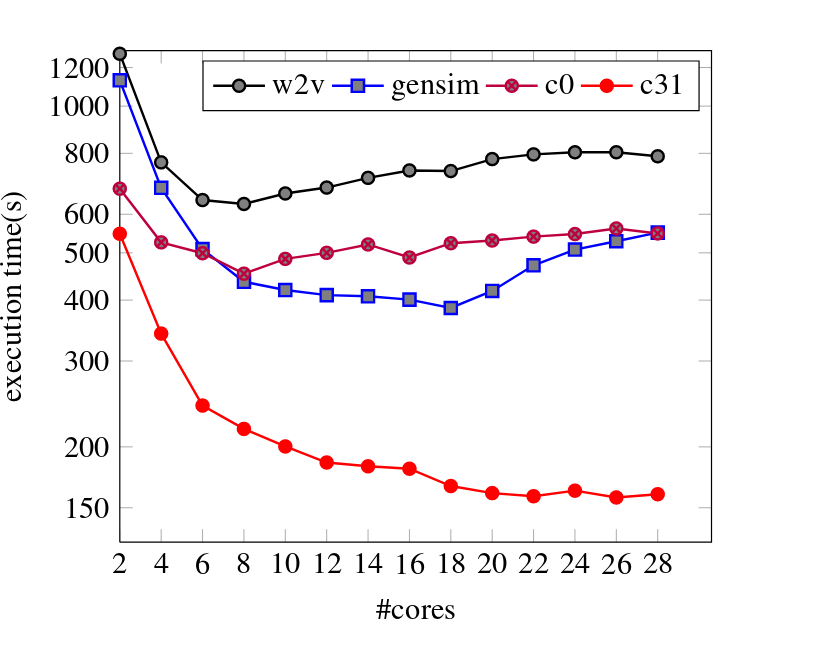
\includegraphics[scale=0.3]{images/cachingEfficiency.png}
\caption{Comparasion of the execution time in relation to the number of used cores \cite{efficient}}
\label{fig:efficient}
\end{figure}
This work proposes a very good way to parallelize the SGM, as in particular, it allows using more cores during the computation. As this approached focused on the Hierarchical softmax, in contrast to our work which uses negative sampling, the next subsection covers optimizations of the Skip-Gram Model with negative sampling(SGNS).

\subsection{Parallization in shared and Distributed Memory}
In contrast to the above approach, this one, introduced by Ji et al. \cite{intel} focused on the SGNS. The focus of this work was to speed up the computation of the loss function of the SGNS described in Equation \ref{eq:obj_neg_samples}. Where the dot product of the center word  with negative samples as well as the context word is computed. The dot product is a level 1-BLAS operation and is not as efficiently implemented into hardware, as matrix multiplication which are a level 3-BLAS operation.  To achieve such a transformation, Ji et al. decided to use the same negative samples for given amount of training samples. The training samples that will have the same negative samples are chosen as follows: given a word $w_c$ one can construct all the training samples where $w_c$ is a context word. The following training batch $X$ will result: $X = \{({w_{in}}^i, w_c) | w_c~appears~in~the~context~of~{w_{in}}^i\}$. The matrix multiplication can be represented in the following way:
\[
\begin{bmatrix}
w_c \\
w_{n_1} \\
\vdots \\
w_{n_k}\\
\end{bmatrix}
*
\begin{bmatrix}
w_{in}^1\\
\vdots\\
{w_{in}}^{2m}\\
\end{bmatrix}
\]
where, $w_{n_1}...w_{n_k}$ are the shared negative samples. The above Matrix multiplication will compute the loss for each training sample and the weights of the used vectors will be updated after each batch. Ji et al.'s method achieves a 3.6 fold increase in throughput, by only losing 1\ % of accuracy. The presented results were achieved on CPU's, as many modern machine learning libraries make use of the parallelizing capabilities of GPU's for matrix multiplications, the next subsection covers the work done by Seulki and Youngmin \cite{gpu} that parellelized the SGNS on GPU's.

\subsection{Accelleration of word2vec by using GPU's}
Seulki and Youngmin \cite{gpu} focused on getting a better throughput on the SGM with the use of GPU's. As the SGM is a sequential algorithm, it is not easy to parallelize it, especially if one wants to parallelize the training of individual training samples. As the algorithm goes sequentially over a sentence, the samples next to each other, in order of execution, will almost every time have the same input word. Consequently, it's very hard to parallelize at this level. 
Since the dimensions of the word embeddings are completly independent of each other  Seulki and Youngmin \cite{gpu} tried to parallelize their update. They achieved this by mapping each dimension to a CUDA thread while mapping each sentence to a CUDA block. As each CUDA block runs independently, the training of the sentences is parallelized, and the fact that sentences have different length is of no problem. If the execution time of the GPU kernel is greater than the time used to read the sentences, it could be a smart choice to use multiple GPU's. According to Seulki and Youngmin \cite{gpu}, if multiple GPU's are used, there is a need for synchronizing the model, which will hinder run time performance. They achieved their best results with 2 concurrent GPU'S. The acomplished results were very good as they managed a 20x speedup compared to a single threaded CPU execution, which is a 3x increase in comparison to the original C code from Mikolov et al. \cite{mikolov2}. The speedup was achieved, while maintaining the accuracy of the model. The problem with this and all the above optimization is that the code is not easily available or of use. Therefore, we need an optimized implementation of the SGM that is easily available. This is provided by Gensim \cite{gensim}, which will be outlined in the next subsection.
%%%%%%%%%%%
\subsection{Gensim}\label{ssec:gensim}
Gensim \cite{gensim} is a pure Python library that holds a state of the art implementation of the SGM. Gensim is written in Cython, which first allowed Gensim to have the same runtime as the original C code. Furthermore, it made use of BLAS's and precomputed sigmoid tables, while also trying to parallelize the training of different sentences. This finally yielded in a 4x speedup in run time compared to the orignal C code from Mikolov et al. Gensim as a python library, and because it was already used in related work \cite{intel} made the comparison easy and of value. \\ This concludes our overview of  related work. The next Section will cover our implementation of the Skip-Gram Model with negative sampling.